\documentclass[tikz,border=8pt]{standalone}
% Shared look for every TikZ diagram. Load with \input{../../tools/tikz-style.tex}
\usepackage[T1]{fontenc}
\usepackage{lmodern}
\renewcommand{\sfdefault}{lmr}  % diagrams use the same serif as the text
\usetikzlibrary{arrows.meta, positioning, shapes.geometric, calc, fit, backgrounds}
\definecolor{cblue}{HTML}{4C78A8}
\definecolor{corange}{HTML}{F58518}
\definecolor{cgreen}{HTML}{54A24B}
\definecolor{cred}{HTML}{E45756}
\definecolor{cpurple}{HTML}{B279A2}
\definecolor{cgrey}{HTML}{6B6B6B}
\tikzset{
  every picture/.style={font=\sffamily, line width=1.2pt},
  box/.style={draw=#1, fill=#1!12, rounded corners=4pt, align=center, inner sep=7pt, minimum height=1.1cm},
  box/.default=cgrey,
  arrow/.style={-{Stealth[length=3mm]}, draw=cgrey, line width=1.4pt},
  title/.style={font=\sffamily\bfseries\Large},
  note/.style={font=\sffamily\small, text=cgrey, align=center},
}
\AtBeginDocument{\hyphenpenalty=10000 \exhyphenpenalty=10000}

\begin{document}
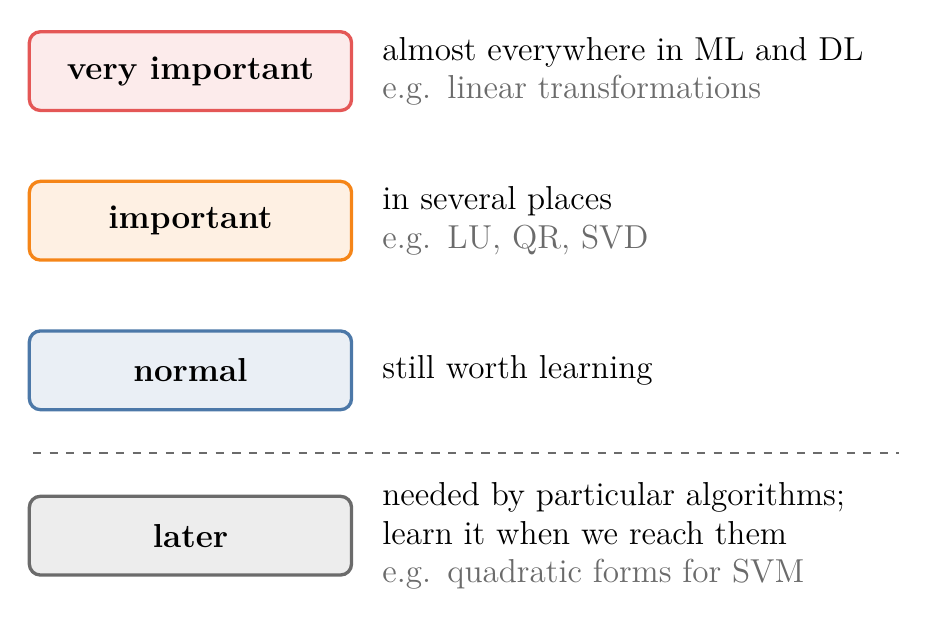
\begin{tikzpicture}[every node/.append style={font=\sffamily\large},
  tag/.style={box=#1, text width=3.6cm, font=\sffamily\bfseries\large, minimum height=1.0cm},
  ex/.style={align=left, text width=6.6cm, anchor=west}]
  \node[tag=cred] (a) at (0,0) {very important};
  \node[ex] at (2.3,0) {almost everywhere in ML and DL\\{\color{cgrey} e.g. linear transformations}};
  \node[tag=corange] (b) at (0,-1.9) {important};
  \node[ex] at (2.3,-1.9) {in several places\\{\color{cgrey} e.g. LU, QR, SVD}};
  \node[tag=cblue] (c) at (0,-3.8) {normal};
  \node[ex] at (2.3,-3.8) {still worth learning};
  \node[tag=cgrey] (d) at (0,-5.9) {later};
  \node[ex] at (2.3,-5.9) {needed by particular algorithms;\\learn it when we reach them\\{\color{cgrey} e.g. quadratic forms for SVM}};
  \draw[cgrey, dashed, line width=1pt] (-2,-4.85) -- (9,-4.85);
\end{tikzpicture}
\end{document}
